\documentclass[11pt]{beamer}
\usetheme{Warsaw}
\usepackage[utf8]{inputenc}
\usepackage[spanish]{babel}
\usepackage{amsmath}
\usepackage{amsfonts}
\usepackage{amssymb}
\usepackage{graphicx}
\usepackage{booktabs}
\author[Juan C. Rabell]{Juan Germán Caltzontzin Rabell\\ Asesor : Dr. Carlos Segura González}
\title[Paisaje de búsqueda en el JSSP]{Paisaje de búsqueda en el problema de planificación de producción tipo taller}
%\setbeamercovered{transparent} 
%\setbeamertemplate{navigation symbols}{} 
%\logo{} 
%\institute{} 
%\date{} 
%\subject{} 
\useoutertheme{split}
\setbeamertemplate{headline}{}
\date{2 de febrero de 2021}
\begin{document}

\begin{frame}
\titlepage
\end{frame}

\begin{frame}
\tableofcontents
\end{frame}

\section{Introducción}
\begin{frame}{Introducción}
En este trabajo se analiza el efecto de distintas metodologías de modificación del paisaje de búsqueda del problema de planificación de producción tipo taller (JSSP por sus siglas en inglés) 
\end{frame}

\begin{frame}{Planteamiento del problema}
Una instancia del JSSP consiste en $n$ trabajos diferentes constituidos cada uno por $m$ operaciones que deben procesarse por un tiempo determinado en $m$ máquinas en una secuencia predeterminada.\\
El objetivo es hallar la planificación que minimiza el tiempo que toma terminar todos los trabajos dado que cada máquina puede procesar solo un trabajo a la vez.
\end{frame}

\begin{frame}{Planteamiento del problema}
Una planificación consiste en asignar tiempos de inicio y fin a cada operación, respetando el orden requerido para cada trabajo. El tiempo que toma terminar todos los trabajos se conoce como makespan y la secuencia de trabajos que toma el mayor tiempo en completarse se conoce como ruta crítica. \\
En general se considera que el tiempo requerido para procesar cada operación puede expresarse como un entero.\\
\end{frame}
\begin{frame}{Ejemplo}
Se muestra un ejemplo de una instancia con 3 máquinas y 2 trabajos.
\begin{table}[H]
\caption{Instancia simple con 3 maquinas y 2 trabajos}
\begin{tabular}{@{}llll@{}}
Trabajo & \multicolumn{3}{l}{\begin{tabular}[c]{@{}l@{}}Secuencia de procesamiento \\ (máquina, tiempo)\end{tabular}} \\ \midrule
0       & 0, 75                              & 2, 54                               & 1, 59                             \\ \midrule
1       & 0, 47                              & 2, 72                              & 1, 45   \\\hline                         
\end{tabular}
\label{tab:inst}
\end{table}
\end{frame}

\begin{frame}{Ejemplo}
La siguiente es una posible planificación para la instancia de ejemplo, visualizada mediante un diagrama de gantt. En negro se marca los trabajos que conforman la ruta crítica. 
\begin{figure}[H]
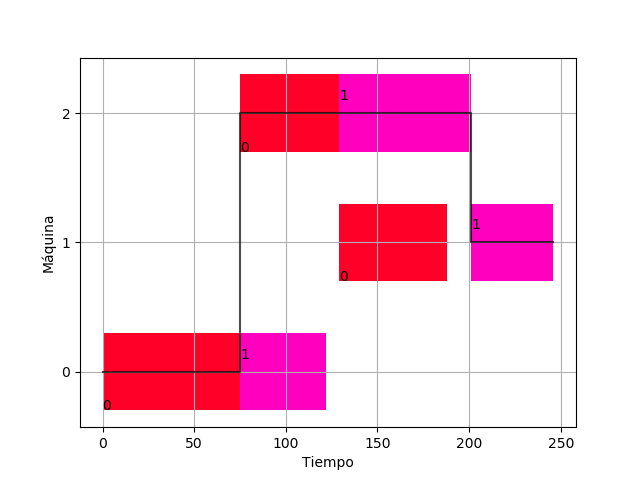
\includegraphics[scale=.5]{planejemplorc.png}
\end{figure}
\end{frame}
\subsection*{Representación de soluciones}
\begin{frame}{Representación de soluciones}
Las soluciones a este problema suelen representarse con una grafo dirigido en el que los nodos son las operaciones de cada trabajo y las aristas representan la secuencia en la que se procesan las operaciones.
El problema de hallar una planificación para cada una de las $m$ operaciones de los $n$ trabajos en las $m$ máquinas se reduce a elegir una permutación de los $n$ trabajos en cada máquina por lo que el número de posibles soluciones es $O(n!^m)$.
\end{frame}
\subsection*{Espacio y paisaje de búsqueda}
\begin{frame}{Espacio de búsqueda}
Una vez que tenemos una representación para las soluciones y operadores de cambio para generar nuevas soluciones a partir de otras, se define el espacio de búsqueda como un grafo dirigido en el que los nodos son las soluciones al problema y una solución $x$ está conectada a otra $y$ si podemos generar a $y$ aplicando los operadores de cambio a $x$.\\
\end{frame}

\begin{frame}{Paisaje de búsqueda}
Podemos asociar a cada solución en el espacio un valor de aptitud o fitness que mide la calidad de dicha solución. La adición de esta función de aptitud al espacio de búsqueda genera al paisaje de búsqueda.
\end{frame}


\begin{frame}{Paisaje de búsqueda}
\begin{figure}
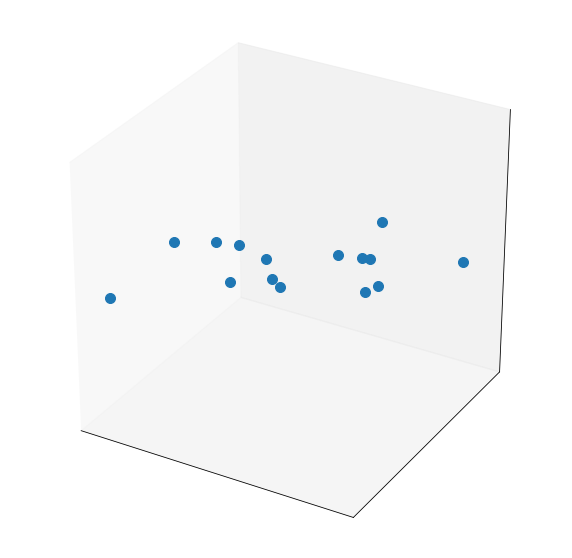
\includegraphics[scale=.4]{search1.png}
\end{figure}
\end{frame}


\begin{frame}{Paisaje de búsqueda}
\begin{figure}
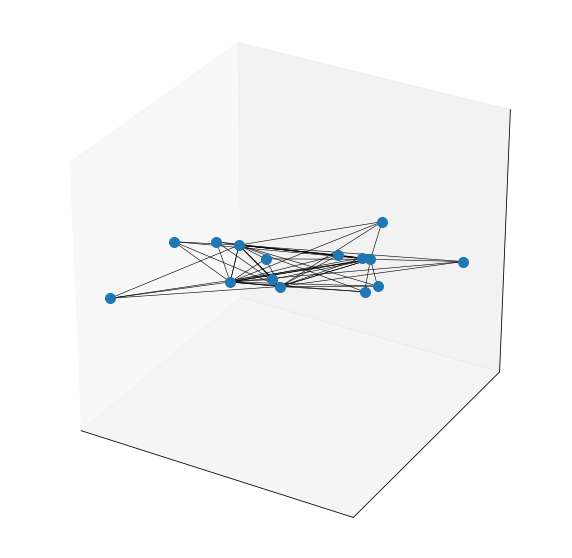
\includegraphics[scale=.4]{search2.png}
\end{figure}
\end{frame}

\begin{frame}{Paisaje de búsqueda}
\begin{figure}
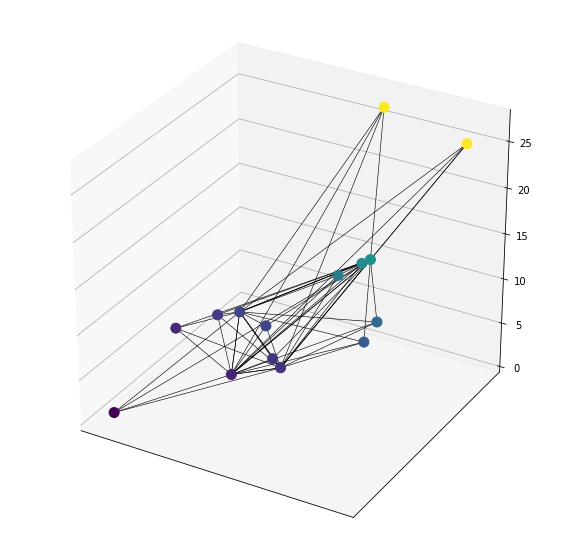
\includegraphics[scale=.4]{search3.png}
\end{figure}
\end{frame}

%\section*{Metaheurísticas}
%\begin{frame}{Metaheurísticas}
%Las metaheurísticas son estrategias de alto nivel que tienen por objetivo encontrar soluciones aceptables en tiempos cortos a problemas que por su tamaño o complejidad no pueden ser resueltos mediante métodos exactos. Para este problema en específico la búsqueda tabú ha dado muy buenos resultados aunque el tiempo que requiere puede llegar a ser del orden de días. 
%\end{frame}

\subsection*{Vecindades}
\begin{frame}{Vecindades}
Para una solución dada al JSSP se define una vecindad como el conjunto de soluciones que se encuentran a una misma distancia de la solución inicial. Esta distancia normalmente se define a partir de los operadores de cambio.
\end{frame}
\begin{frame}{Vecindades}
Para este problema se han planteado varias estructuras de vecindad a partir de la denominada ruta crítica de la solución. La ruta crítica es la secuencia de trabajos más larga en la planificación. Puede probarse que para reducir el makespan de una solución necesariamente tienen que intercambiarse al menos dos operaciones que pertenezcan a la ruta crítica. La vecindad con la que se han obtenido los resultados del estado del arte se conoce como N7.
\end{frame}


%\subsection*{Búsqueda local iterada}
%\begin{frame}{ILS}
%Para intentar disminuir el tiempo necesario para obtener soluciones aceptables se implementó la búsqueda local iterada (ILS por sus siglas en inglés) que consiste en realizar una búsqueda local en alguna vecindad y cambiar a un vecino mejor que la solución actual hasta que encontremos un mínimo local, una vez que se ha obtenido esta solución se le aplica una perturbación y se repite el proceso hasta cumplir algún criterio de paro (e.g. el tiempo).
%\end{frame}
%
%\begin{frame}{Perturbación}
%En la ILS el operador de perturbación juega un papel muy importante en la exploración del espacio de búsqueda. Es importante poder perturbar la solución de una manera que nos permita salir de mínimos locales sin perder demasiado la estructura de la solución.
%\end{frame}
%
%\begin{frame}{Deficiencias de la ILS}
%Para este problema la ILS tiene la desventaja de estancarse en mínimos locales malos. Para intentar disminuir este problema se pueden tomar varias rutas de acción, en concreto se tomaron dos: considerar una vecindad más grande y modificar la función objetivo con el objetivo de poder aceptar cambios que no generen una disminución directa en el makespan pero mejoren otras características de la solución.
%\end{frame}
\section*{Objetivo y motivación}
\begin{frame}{Objetivo y motivación}
Actualmente los resultados del estado del arte para este problema se han obtenido mediante algoritmos meméticos con búsqueda tabú y con ejecuciones de entre 24 y 48 hrs paralelas.\\
La literatura reciente se ha centrado en hacer más eficiente la búsqueda tabú sin considerar el paisaje de búsqueda.\\
El objetivo de este trabajo es plantear modificaciones que permitan el uso de mecanismos más simples y rápidos para encontrar soluciones comparables al estado del arte.
\end{frame}
\section*{Hipótesis}

\begin{frame}{Hipótesis}
Es posible conseguir resultados comparables al estado del arte con algoritmos sencillos y rápidos si modificamos el paisaje de búsqueda.\\
\end{frame}

\section*{Propuestas}
\begin{frame}{Propuestas}
\begin{enumerate}
\item Se propone utilizar la búsqueda local iterada (ILS por sus siglas en inglés) por ser un algoritmo simple y rápido.
\item Se propone una extensión a la vecindad N7
\item Se planteó una función de fitness que no solo toma en  cuenta el makespan sino también los tiempos de finalización de todas las máquinas.
\end{enumerate}
\end{frame}
%\section{Problemas de benchmark}
%\begin{frame}{Benchmarks}
%Se tienen varios conjuntos de problemas como benchmark, en este trabajo se utilizan las instancias dmu propuestas por Ebru Demirkol, Sanjay Mehta y Reha Uzsoy que consisten en 80 problemas que tienen desde 20 trabajos y 15 máquinas ($20\times 15$) hasta 50 trabajos y 20 máquinas ($50\times 20$).   
%\end{frame}
\section{Resultados}
\begin{frame}{Resultados}
Aquí se presentan los resultados de las dos variantes de ILS, modificar la función objetivo y agrandar la vecindad. También se muestran los mejores resultados reportados a la fecha en la literatura para 80 instancias de prueba comúnmente utilizadas. Las 80 instancias se muestran en dos partes. A cada instancia se le aplicó ILS por 5 min, para 100 soluciones generadas aleatoriamente. Se muestran los mejores resultados obtenidos.
\end{frame}

\begin{frame}{Resultados}
\begin{figure}
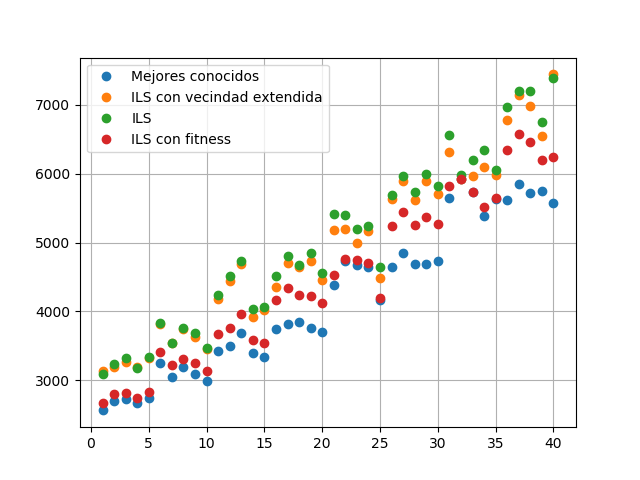
\includegraphics[scale=.6]{bestres/best1.png}
\caption{Resultados de cada método en la primer mitad de instancias}
\end{figure}
\end{frame}

\begin{frame}{Resultados}
\begin{figure}
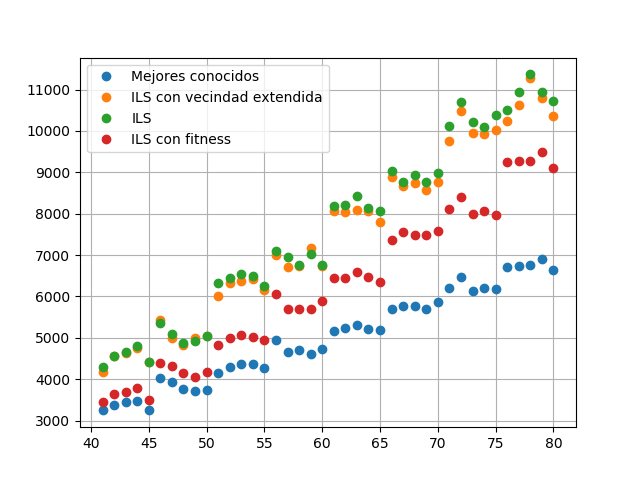
\includegraphics[scale=.6]{bestres/best2.png}
\caption{Resultados de cada método en la segunda mitad de instancias}
\end{figure}
\end{frame}

\section{Conclusiones}
\begin{frame}{Conclusiones}
La modificación de la función objetivo obtuvo mejores resultados que la extensión de vecindad aunque ambos presentan una mejora respecto a la ILS sin modificaciones.\\
La segunda mitad de las instancias utilizadas tienen una estructura en la que es más fácil estancarse en óptimos locales de peor calidad.\\
\end{frame}

\begin{frame}{Trabajo a futuro}
\begin{figure}
\centering
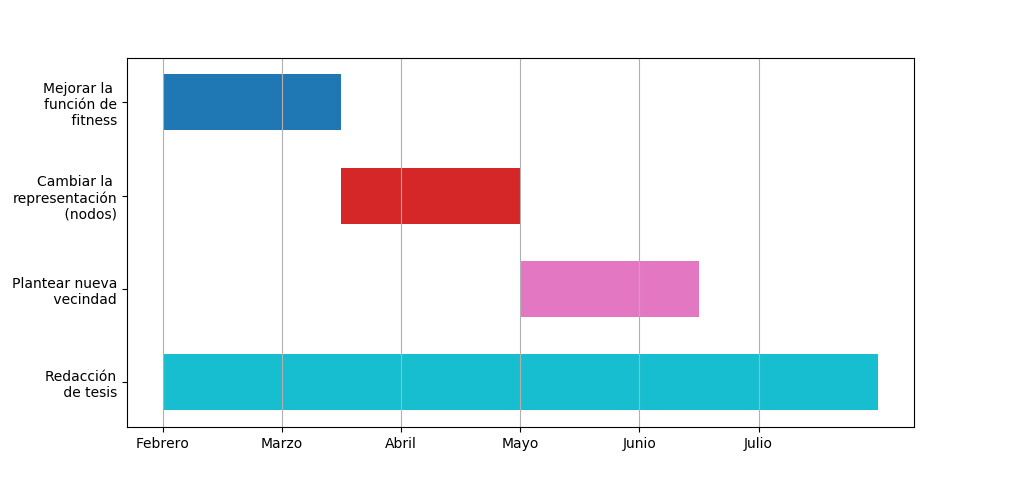
\includegraphics[scale=.46]{plantesis.png}
\end{figure}
\end{frame}
\end{document}